\chapter{Electrical Design}
\section{Introduction}
The electronics of the robot use a combination of off-the-shelf parts and custom designed circuits. 


\section{Power}
A four cell, 1800 mAH lithium polymer (LiPo) battery powers the entire system. The battery is connected using polarized XT60 connectors to prevent reverse connection. The battery voltage varies between 16.8 V when fully charged and 14.8 V when depleted so two off-the-shelf DC-DC buck regulators, shown in Figure \ref{fig:smps} buck battery voltage down to 12 V and 7 V supplies. The switching regulators accept a 7 -- 40 V supply and can output 1.2 -- 35 V at 8 A each. The 12 V bus powers the three motor drivers boards while the 7 V bus powers the STM32 Nucleo-64 development board and two AZ1085CD low-dropout linear regulators (LDO). One LDO produces a 5 V bus while the other provides 3.3 V, each at 3 A. 

\begin{figure}[H]   % [h] means here
	\centering 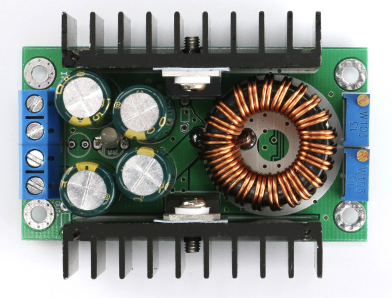
\includegraphics[width=6in, height=3.85in, keepaspectratio]{figures/smps.png}
	\caption{DC-DC Buck Regulator \cite{smps}}\label{fig:smps}
\end{figure}

\section{Sensors}



\section{Motor Drivers}
The system uses three off-the-shelf L298N motor driver boards since they are easily obtainable for less than \$6 each and incorporate features such as heat-sinking, flyback voltage protection, supply filtering, and screw terminal connections. Implementing comparable motor drivers with a similar feature set would undoubtedly cost more. Each L298N is a dual H-bridge driver with 2 A maximum output per bridge using a 5 -- 35 V supply. Two motor drivers handle the four robot drive motors while the third powers the blower fan and shooting mechanism motors. 

Figure \ref{fig:l298n} shows a wiring diagram for each motor driver. The board uses four digital control inputs, each controlling the state of one half-bridge. Each motor uses a pair of inputs: IN1 and IN2 control one motor while IN3 and IN4 control the other. To achieve direction and speed control, IN1 and IN3 are pulse width modulated (PWM) while IN2 and IN4 are digitally set. Table \ref{tab:L298N_truth_table} is a truth table of the motor state versus inputs.

\begin{figure}[H]   % [h] means here
	\centering 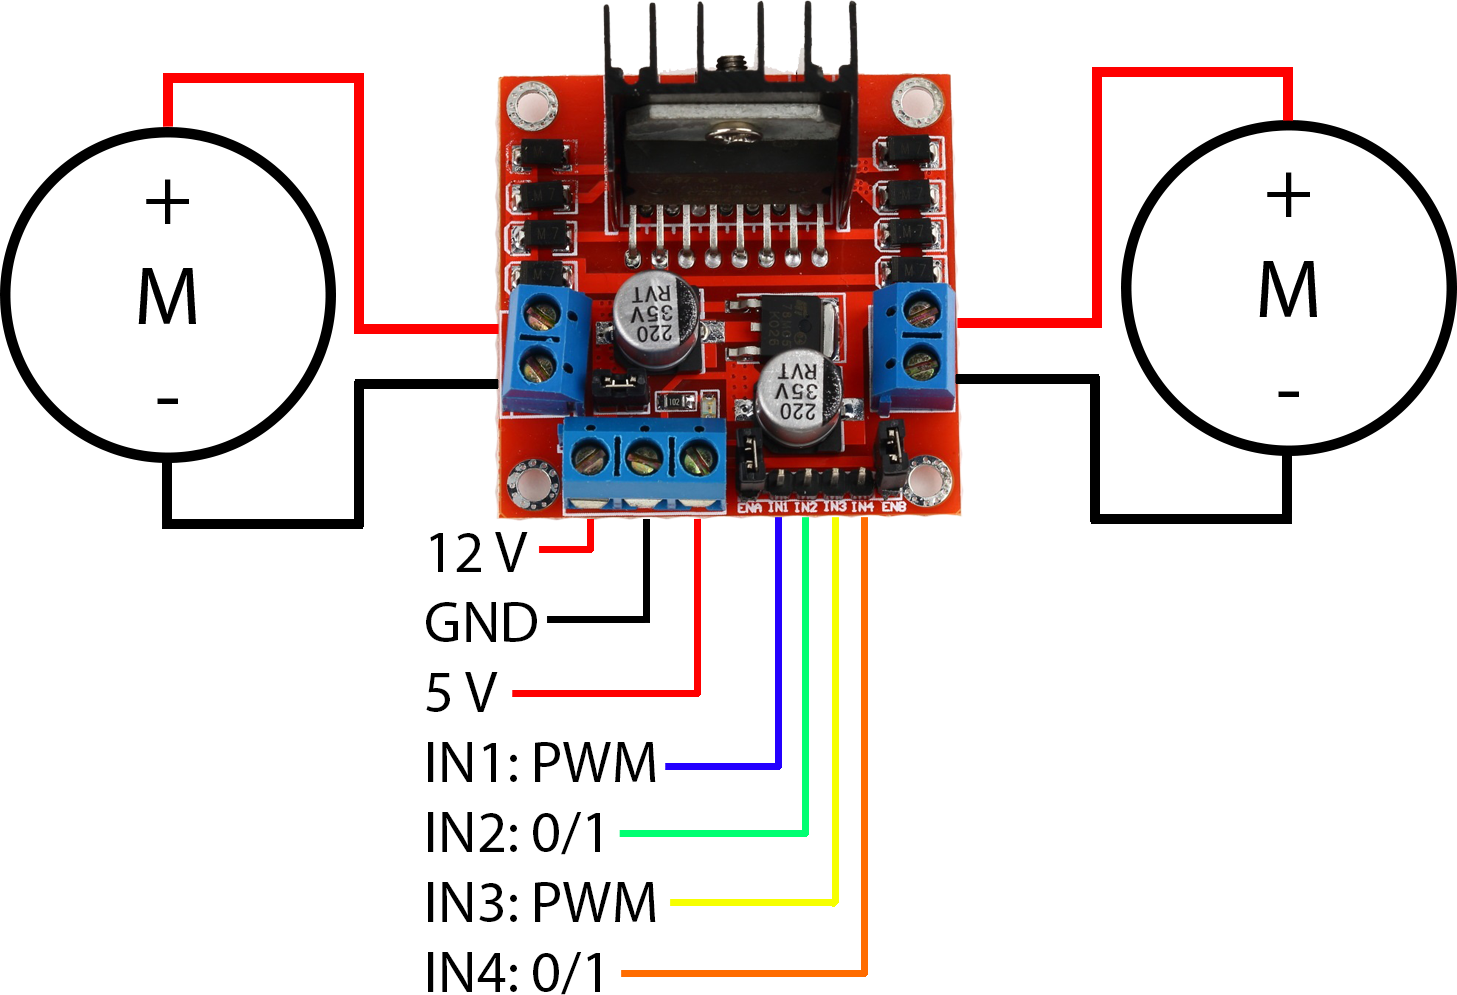
\includegraphics[width=6in, height=3.85in, keepaspectratio]{figures/l298n.png}
	\caption{L298N Motor Driver Wiring Diagram \cite{l298n}}\label{fig:l298n}
\end{figure}

\begin{table}[h]
	\centering	\caption{Motor Control Truth Table}
	\begin{tabular}{ccc}
		\hline 
		IN1/IN3 Duty Cycle & IN2/IN4 State & Motor State \\ 
		\hline 
		0\% & 0 & Stopped \\ 
		\hline 
		\textgreater 0\% & 0 & Forward, speed increases with duty cycle \\ 
		\hline 
		\textless 100\% & 1 & Reverse, speed decreases with duty cycle \\ 
		\hline 
		100\% & 1 & Stopped \\ 
		\hline 
	\end{tabular} 
	\label{tab:L298N_truth_table}
\end{table}

\section{Interconnect PCB}

\subsection{Schematic Capture}

\subsection{Board Layout}

\subsection{Assembly}

\subsection{Reworks}